\documentclass[article, a2paper, oneside, landscape]{memoir}
\usepackage{tikz}
\usetikzlibrary{mindmap}
\pagestyle{empty}

\begin{document}
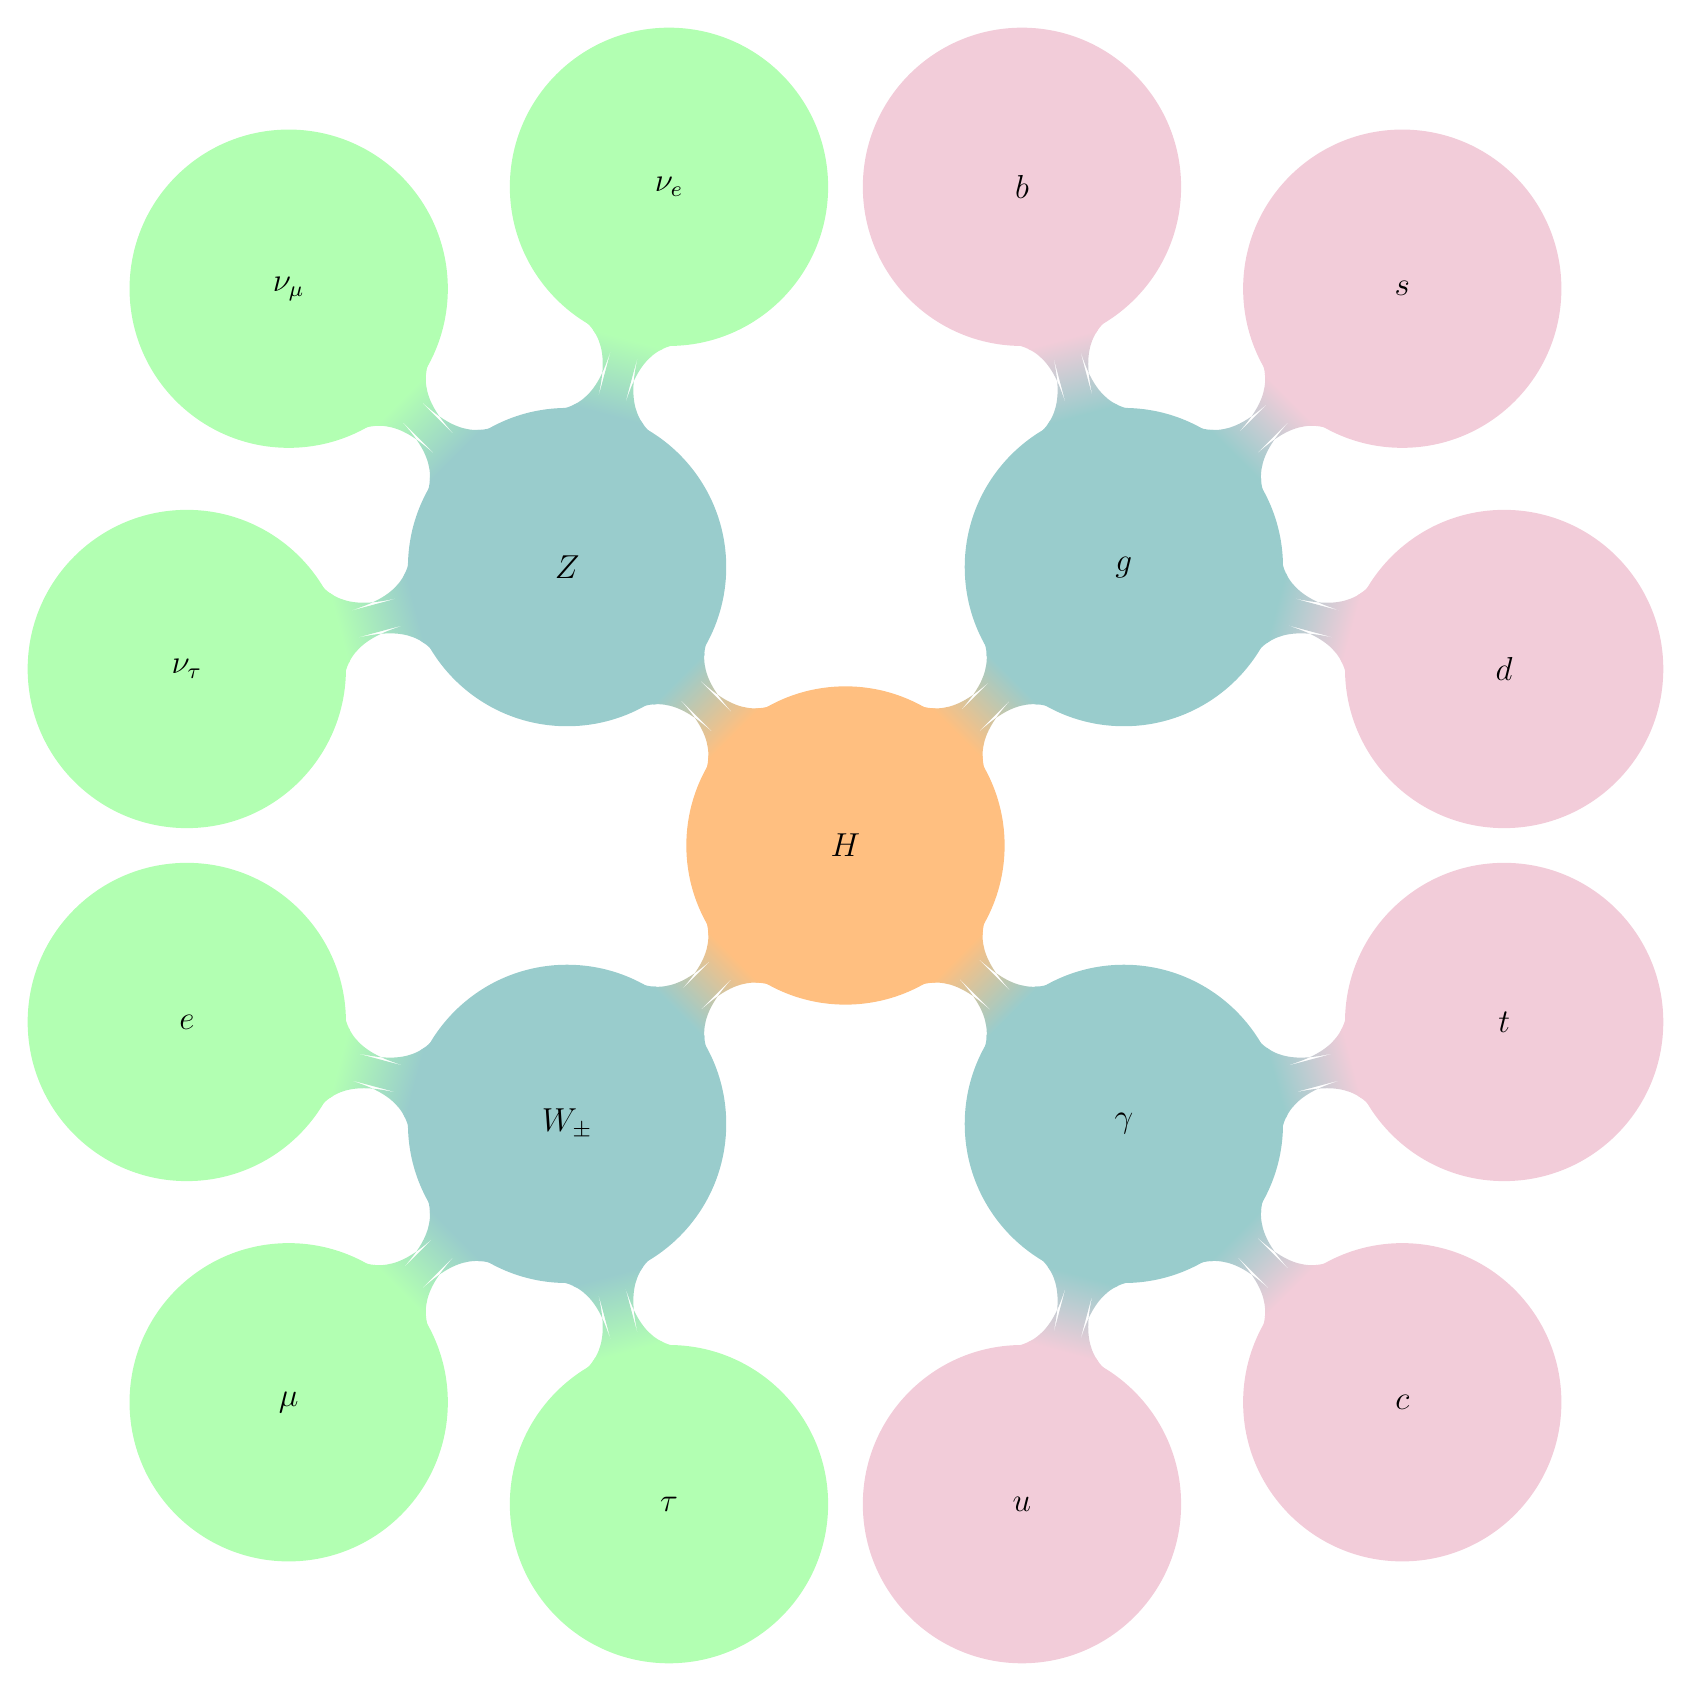
\begin{tikzpicture}[mindmap, grow cyclic, every node/.style=concept, concept color=orange!50,
  level 2/.style={level distance=5cm,sibling angle=60},
  level 1/.style={level distance=5cm,sibling angle=90}]

\node{$H$}
  child [concept color=teal!40] { node {$W_{\pm}$}
    child [concept color=green!30] { node {$e$}}
    child [concept color=green!30] { node {$\mu$}}
    child [concept color=green!30] { node {$\tau$}}
  }
  child [concept color=teal!40] { node {$\gamma$}
    child [concept color=purple!20] { node {$u$}}
    child [concept color=purple!20] { node {$c$}}
    child [concept color=purple!20] { node {$t$}}
  }
  child [concept color=teal!40] { node {$g$}
    child [concept color=purple!20] { node {$d$}}
    child [concept color=purple!20] { node {$s$}}
    child [concept color=purple!20] { node {$b$}}
  }
  child [concept color=teal!40] { node {$Z$}
    child [concept color=green!30] { node {$\nu_e$}}
    child [concept color=green!30] { node {$\nu_\mu$}}
    child [concept color=green!30] { node {$\nu_\tau$}}
  }
;

\end{tikzpicture}
\end{document}
